%% Consignes : parties prenantes / responsabilites ; ressources materielles,
%% humaines et financieres ; planification / phases et jalons ; risques.

\subsection{Stakeholders and Responsibilities}
\label{sec:parties_prenantes}

The mission was carried out inside a small research team, and the distribution of
responsibility mattered more than its size suggests. Table~\ref{tab:parties} lists who did
what.

\begin{table}[htbp]
\centering
\caption{Stakeholders and their role in the mission}
\label{tab:parties}
\small
\begin{tabularx}{\linewidth}{>{\raggedright\arraybackslash}p{3.7cm} >{\raggedright\arraybackslash}p{3.6cm} X}
\toprule
\textbf{Person} & \textbf{Role} & \textbf{Responsibility in this mission} \\
\midrule
S\'ebastien Perthuisot & Research Programme Director, Quality \& Supply Chain Expert &
Set the research direction, arbitrated scope, chaired the weekly regular point and the
Friday demonstration. Decision-maker on what the programme keeps. \\
\'Emilienne Lardy & Scientific supervision & Ran the Monday planning and the three weekly
scrums; reviewed method and written output. First reader of anything claimed. \\
Selma Ferhat & Scientific supervision & Reviewed the scientific framing and the written
record. \\
Fabien Jules & Charg\'e Innovation & Placement tutor of record; onboarding, administrative
framing and access. \\
Liam Jones & Fellow intern, same programme & Network representation, graph modelling and
geographic layer of the twin. Neighbouring problem, shared demonstration slot. \\
David Gomez & ESTIA academic supervisor & Academic framing of the mission. \\
Author & Intern, Supply Chain Engineer & Model, implementation, experimental design,
analysis and written deliverables. \\
\bottomrule
\end{tabularx}
\end{table}

The presence of a second intern on an adjacent problem shaped the work more than expected.
Liam Jones was building the structural and geographic representation of a supply chain,
meaning how a network is described, generated and visualised, while this mission built the
layer that scores nodes once they exist. The two are complementary halves of the same twin,
and the Friday demonstration forced each to state weekly what the other could rely on. It
also produced a boundary decision early: the scoring layer would assume a network is given
rather than attempt to generate one, because that was being solved two seats away.

\subsection{Resources}
\label{sec:ressources}

The resources provided were modest and are worth stating plainly, because two of them
constrained technical choices.

\begin{itemize}
    \item \emph{Human.} No budget-holding team. Supervision as listed above, and one peer on
    an adjacent subject. All implementation was carried out by the author.
    \item \emph{Material.} One laptop provided by ALTEN, a Ryzen~7 PRO 8840HS with 16 cores
    and no discrete GPU. Everything computed in this mission, including every model training
    run, ran on that CPU.
    \item \emph{Software.} Azure DevOps for source control and work tracking, and the
    Microsoft suite for communication. No paid data service, no cloud compute budget, no
    commercial solver or licence was requested or used, which is why the delivered system
    depends only on open-source Python libraries and a file-based database.
    \item \emph{Financial.} None directly managed. The absence of a budget is itself a
    design constraint: it removed managed cloud services and paid datasets from the solution
    space before any technical comparison took place.
\end{itemize}

\subsection{Working Method: Agile and Test and Learn}
\label{sec:methode}

The placement agreement prescribes an evolutionary approach based on Agile and Test and
Learn. That was applied literally rather than nominally, and the weekly rhythm was the
mechanism.

\paragraph{The cadence.}
The week had a fixed shape. A planning session on Monday set the objective for the week. A
scrum on Tuesday, Wednesday and Thursday morning kept it visible and surfaced blockages
within a day rather than a week. A regular point with the programme director on Wednesday
took the scientific decisions. A demonstration on Friday closed the loop by requiring
something to be shown, not described. Four contact points a week on a six-month mission is a
heavy cadence for R\&D, and it was the single most useful organisational feature of the
placement: it made it impossible to spend three weeks on an idea that would not survive
contact with a reviewer.

\paragraph{Test and Learn, with what it actually rejected.}
The method is only meaningful if things were genuinely abandoned. Four were.

\begin{enumerate}
    \item \emph{The first urgency formulation was dropped.} The initial model expressed
    urgency as a single time-driven function with a finite-time singularity, calibrated by
    penalty terms. It was specified, partially implemented and abandoned in favour of a
    multi-block aggregation, because a single deadline-proximity curve discards information
    the twin already holds and cannot represent a node that is on time but out of capacity.
    \item \emph{The May module architecture was replaced.} A first pipeline of separate
    scores was built through May and superseded in June by the aggregation and propagation
    design that shipped. The intermediate work was not wasted: it established what the
    interfaces between components needed to be, which is why the replacement was built in
    weeks rather than months.
    \item \emph{A candidate dataset was rejected on inspection.} A third-party logistics
    dataset considered for the freight node was checked before use and discarded: it carried
    pre-computed target columns, coordinates scattered outside the region it claimed to
    cover, and uniformly flat distributions, all signatures of synthetic data. The node was
    driven by calibrated events instead. The rejected file is retained for audit and never
    loaded by the analysis pipeline.
    \item \emph{A whole experimental arm was reduced.} The campaign was designed for eight
    human consultants over nine working days. When that could not be secured, the design was
    changed rather than the claim: the campaign was run with isolated agents, and every
    conclusion about human behaviour was correspondingly weakened in the reporting.
\end{enumerate}

\begin{figure}[htbp]
    \centering
    \includegraphics[width=0.72\linewidth]{Images/4.Operations/test_learn_loop.png}
    \caption{The test-and-learn iteration loop}
    \label{fig:testlearn}
\end{figure}

Figure~\ref{fig:testlearn} shows the loop as it was actually run. Each turn of it produced
either a working increment or a documented rejection, and the four rejections above are the
evidence that the second outcome was genuinely available rather than theoretical.

\paragraph{Quality gates.}
Agile without a definition of done produces velocity and nothing else. Three gates were
applied: no feature merged without automated tests, giving 1\,779 test functions at the end
of the mission; every business write passing through a single audited mutation service, so
that no result could be produced by an untraceable edit; and every reported figure
regenerated from raw artefacts by a script rather than transcribed by hand.

\subsection{Phases and Milestones}
\label{sec:planning}

The mission ran in six phases. Figure~\ref{fig:gantt} gives the schedule and
Table~\ref{tab:jalons} the milestones that closed each phase.

\begin{figure}[htbp]
    \centering
    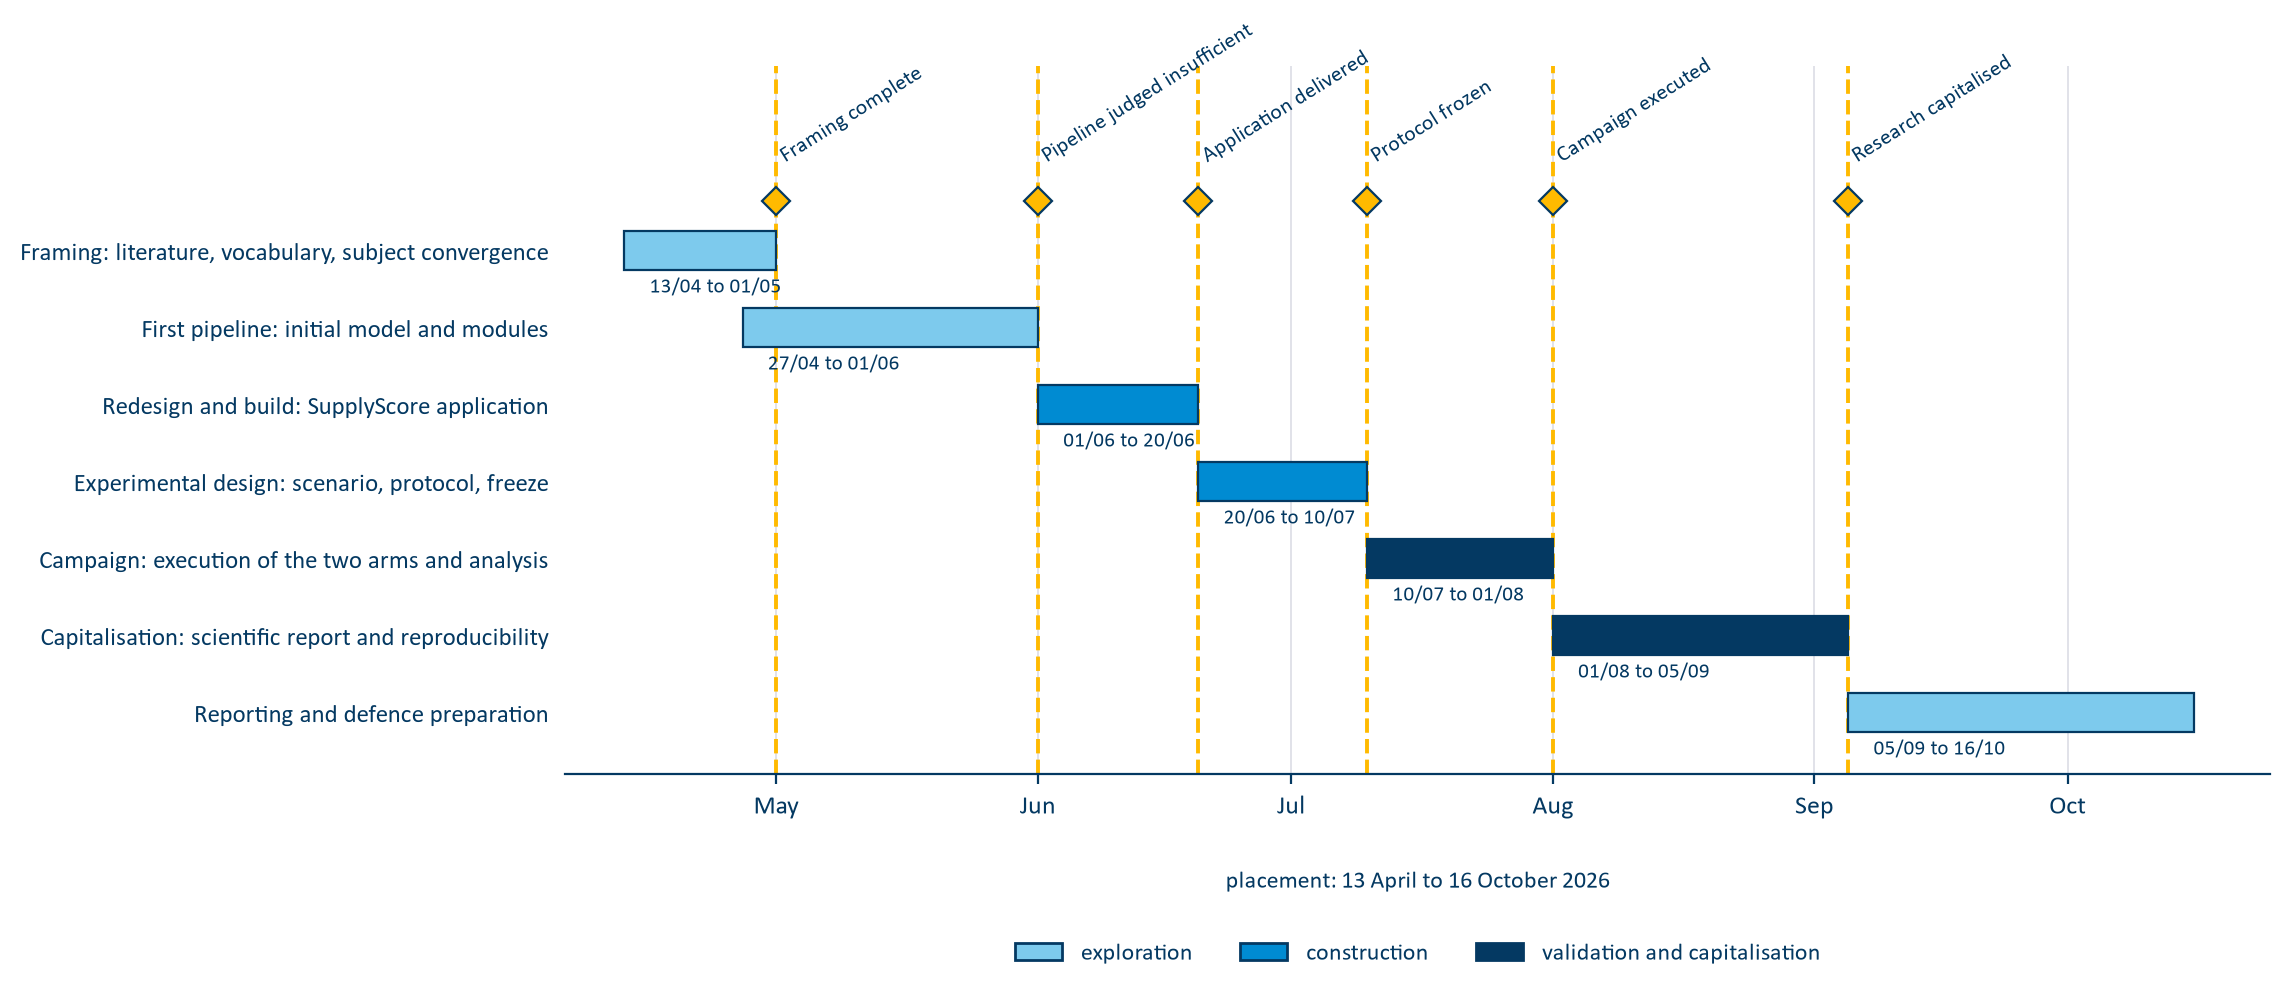
\includegraphics[width=0.96\linewidth]{Images/gantt.png}
    \caption{Phases and milestones of the mission}
    \label{fig:gantt}
\end{figure}

\begin{table}[htbp]
\centering
\caption{Milestones}
\label{tab:jalons}
\small
\begin{tabularx}{\linewidth}{>{\raggedright\arraybackslash}p{2.4cm} >{\raggedright\arraybackslash}p{3.4cm} X}
\toprule
\textbf{Date} & \textbf{Milestone} & \textbf{Closed by} \\
\midrule
End April & Framing complete & Knowledge transfer report and state of the art presented;
subject converged with the programme director \\
End May & First pipeline & End-to-end computation running, and found insufficient, which
triggered the redesign \\
Mid June & Application delivered & Multi-tenant persistence, audited writes, weekly cycle,
event engine, explainability, exports and backup \\
Early July & Protocol frozen & Scenario, data pack hashed, role cards and hypothesis
register registered before any data existed \\
End July & Campaign executed & Two arms run, analysed against the pre-registered register \\
Mid August & Research capitalised & Scientific report and reproducible derivation of every
figure \\
\bottomrule
\end{tabularx}
\end{table}

The planning was revised once, in June. The original schedule allocated the second half of
the mission to extending the model's scope; it was reallocated to validating what already
existed, on the argument that an unvalidated extension of an unvalidated model compounds the
problem rather than advancing it. That reallocation is the reason this report can state a
measured result at all.

\subsection{Risks and Mitigations}
\label{sec:risques}

Four risks were identified and carried at the start of the mission.
Table~
\ref{tab:risques} states each one, whether it materialised, and what was done about
it. Three of the four did materialise, which is a high rate and reflects how much of this
mission depended on things outside the author's control.

\begin{table}[htbp]
\centering
\caption{Risk register and outcomes}
\label{tab:risques}
\small
\begin{tabularx}{\linewidth}{>{\raggedright\arraybackslash}p{3.5cm} >{\raggedright\arraybackslash}p{1.8cm} X}
\toprule
\textbf{Risk} & \textbf{Outcome} & \textbf{Mitigation and effect} \\
\midrule
No access to academic literature from within ALTEN & Materialised & The Direction de
l'Innovation holds no journal or database subscriptions, so a state of the art conducted
from the company alone would have rested on whatever is publicly readable. The mission
depended throughout on ESTIA and Cranfield library credentials. It worked, but the
dependency is real and would block a consultant without a university affiliation. \\[3pt]
\midrule
Broad mission scope & Materialised & Five workstreams in the signed assignment against one
person and six months. Mitigated by converging the subject in the first weeks with the
programme director and recording the boundaries explicitly
(Section~\ref{sec:mission_perimetre}) rather than leaving them implicit. \\[3pt]
\midrule
Human campaign might not be securable & Materialised & Eight colleagues for nine working
days was never guaranteed. Mitigated by designing the protocol so that the declarant could
be substituted without changing the record format, which is what allowed the campaign to run
at all when the humans were unavailable. Cost: the external validity of every behavioural
claim. \\[3pt]
\midrule
CPU-only compute & Contained & No GPU available. Bounded model size and training resolution,
and is the reason one comparison was run at reduced scale. Mitigated by choosing methods
whose cost is dominated by data rather than by parameters. \\
\bottomrule
\end{tabularx}
\end{table}

The first risk deserves a comment, because it is the one least often written down. An R\&D
department that cannot read the literature it is meant to advance is dependent on the
academic affiliations of the people passing through it. For a placement holder on a double
degree that is invisible, since the credentials come with the student. It stops being
invisible the moment the work has to be continued by someone without them, which is a
succession risk for the programme rather than a problem for this mission.
